% cpedoc.tex V2.0, 13 May 2010

\documentclass[times]{cpeauth}

\usepackage{moreverb}
\usepackage{xspace}

\newif\ifdraft
%\drafttrue
\ifdraft
\newcommand{\onote}[1]{ {\textcolor{cyan} { (***Ole: #1) }}}
\newcommand{\terminology}[1]{ {\textcolor{red} {(Terminology used: \textbf{#1}) }}}
\newcommand{\owave}[1]{ {\cyanuwave{#1}}}
\newcommand{\jwave}[1]{ {\reduwave{#1}}}
\newcommand{\alwave}[1]{ {\blueuwave{#1}}}
\newcommand{\jhanote}[1]{ {\textcolor{red} { ***shantenu: #1 }}}
\newcommand{\alnote}[1]{ {\textcolor{green} { ***andreL: #1 }}}
\newcommand{\amnote}[1]{ {\textcolor{blue} { ***andreM: #1 }}}
\newcommand{\smnote}[1]{ {\textcolor{brown} { ***sharath: #1 }}}
\newcommand{\pmnote}[1]{ {\textcolor{brown} { ***Pradeep: #1 }}}
\newcommand{\msnote}[1]{ {\textcolor{cyan} { ***mark: #1 }}}
\newcommand{\note}[1]{ {\textcolor{magenta} { ***Note: #1 }}}
\else
\newcommand{\onote}[1]{}
\newcommand{\terminology}[1]{}
\newcommand{\owave}[1]{#1}
\newcommand{\jwave}[1]{#1}
\newcommand{\alnote}[1]{}
\newcommand{\amnote}[1]{}
\newcommand{\athotanote}[1]{}
\newcommand{\smnote}[1]{}
\newcommand{\pmnote}[1]{}
\newcommand{\jhanote}[1]{}
\newcommand{\msnote}[1]{}
\newcommand{\note}[1]{}
\fi

\newcommand{\pilot}{Pilot\xspace}
\newcommand{\pilots}{Pilots\xspace}
\newcommand{\pilotjob}{Pilot-Job\xspace}
\newcommand{\pilotjobs}{Pilot-Jobs\xspace}
\newcommand{\pilotcompute}{Pilot-Compute\xspace}
\newcommand{\pilotmapreduce}{PilotMapReduce\xspace}
\newcommand{\pilotdata}{Pilot-Data\xspace}
\newcommand{\pd}{PD\xspace}
\newcommand{\pj}{PJ\xspace}
\newcommand{\pjs}{PJs\xspace}
\newcommand{\pds}{Pilot Data Service\xspace}
\newcommand{\computeunit}{Compute-Unit\xspace}
\newcommand{\computeunits}{Compute-Units\xspace}
\newcommand{\dataunit}{Data-Unit\xspace}
\newcommand{\dataunits}{Data-Units\xspace}
\newcommand{\du}{DU\xspace}
\newcommand{\dus}{DUs\xspace}
\newcommand{\cu}{CU\xspace}
\newcommand{\cus}{CUs\xspace}
\newcommand{\su}{SU\xspace}
\newcommand{\sus}{SUs\xspace}
\newcommand{\schedulableunit}{Schedulable Unit\xspace}
\newcommand{\schedulableunits}{Schedulable Units\xspace}
\newcommand{\cc}{c\&c\xspace}
\newcommand{\CC}{C\&C\xspace}

\usepackage[
%dvips,
colorlinks,bookmarksopen,bookmarksnumbered,citecolor=red,urlcolor=red]{hyperref}

\newcommand\BibTeX{{\rmfamily B\kern-.05em \textsc{i\kern-.025em b}\kern-.08em
T\kern-.1667em\lower.7ex\hbox{E}\kern-.125emX}}

\def\volumeyear{2012}



\begin{document}

\runningheads{S. Jha et al.}{Pilot-Abstractions for MapReduce-based Applications on Clouds and Grids}

\title{Extensible, Scalable, Interoperable Pilot-Abstractions for MapReduce-based Applications on Clouds and Grids}

\author{Melissa Romanus, Andre Luckow, Pradeep Mantha, Shantenu Jha\corrauth}

\address{Radical Research Group, Rutgers University}

\corraddr{Journals Production Department, John Wiley \& Sons, Ltd,
The Atrium, Southern Gate, Chichester, West Sussex, PO19~8SQ, UK.}

\begin{abstract}

The data generated by scientific applications is experiencing an exponential
growth. The efficient use of distributed resources will be the key to making
meaningful sense of all of the data produced. In our recent work we showed how
MapReduce can be used to efficiently process distributed data across on a
distributed set of resources. \pilotmapreduce 
(PMR)~\cite{Mantha:2012:PEF:2287016.2287020} is a flexible,
infrastructure-independent runtime environment for MapReduce. PMR is based on
Pilot-abstractions for compute (Pilot-Jobs) and data (Pilot-Data). Pilot-Jobs
are used to couple the map phase computation to the nearby source data, and
Pilot-Data is used to move intermediate data using parallel data transfers to
the reduce computation phase.

In this work, we show how Pilot abstractions and PMR enable the processing of
distributed data across multiple heterogeneous distributed infrastructure,
including concurrent usage of clouds and traditional grids/clusters. We 
further show how PMR can efficiently support different infrastructure 
and application characteristics, e.\,g.\ applications that
require iterative MapReduce. We further analyze different resource topologies
and MapReduce configuration, such as both hierarchical and iterative 
MapReduce. In particular, we investigate typical infrastructure trade-offs 
(e.g. the overhead times in spawning virtual machines, the
geographic distribution, etc). 

\end{abstract}

\keywords{MapReduce; Grid Computing; Cloud Computing; K-Means; Data-Intensive; Compute-Intensive}

\maketitle

\footnotetext[2]{Please ensure that you use the most up to date
class file,
available from the CPE Home Page at\\
\href{http://www3.interscience.wiley.com/journal/117946197/grouphome/home.html}{\texttt{http://www3.interscience.wiley.com/journal/117946197/grouphome/home.html}}}

\vspace{-6pt}

\section{Introduction}
\vspace{-2pt}
Motivation of problem in scaling data intensive applications- 
Interoperability, Scalability, Extensibility/Flexibility/usability.

   - Why is this a problem? Any real application requires this problem to be solved?

   - CMS, Atlas generates PBs of data/ day.

Why Iterative MapReduce?

What Application?  ( k-means?)

Why k-means?

  - twister mapreduce used k-means?

  - k-means implemented using windows azure




Some Research Questions?
 
Can we say something when to use cloud or When Grid ? 
Does minimizing queue wait time, distributed nature of Pilot-abstractions motivate Domain Scientists to use freely available Grid resources? 
Waiting time and cost increases as Number of instances required increase? 
HOw is it beneficial than Grids? 

Why Domain scientists are moving to cloud? Hype? Due to non-availability of necessary simple abstractions to scale applications on Grid?


\section{Related Work}


\section{Distributed Storage Infrastructure}

In distributed settings, storage is often a black box for the application with
unknown quality of services, i.\,e. the application usually does not know what
bandwidths and latencies it can expect. Furthermore, physical and logical
distribution implies higher penalties for inefficient data access as the data
traverses several hardware and software layers.

In general, different types of storage exist (see 
figure~\ref{fig:figures_storage-types}):

\begin{enumerate}
	\item \textbf{Local Storage:} describes local hard disk directly attached 
	to the compute resource.
	\item \textbf{Network Filesystem:} refers to different forms of 
	distributed (possible parallel) filesystems. The filesystem is commonly 
	exported via the Posix API and a virtual filesystem layer.
	\item \textbf{Distributed Storage:} refers to a highly distributed type of 
	storage systems that spawn across multiple data centers. Access to such 
	storage systems via a common -- often simplified -- namespace and API. For 
	example, cloud systems, such as the Azure Blob Storage, Amazon S3 and 
	Google Storage, provide only a namespace with a 1-level hierarchy. 
\end{enumerate}

While the coupling between compute and data in type 1 and 2 is very high, it 
is only small in the later case. In general, the buffer type 3 storage are 
more optimized to reliably storing large volumes of data and achieving high
read throughputs.

\alnote{Why do we exclude databases?}

\begin{figure}[t]
	\centering
		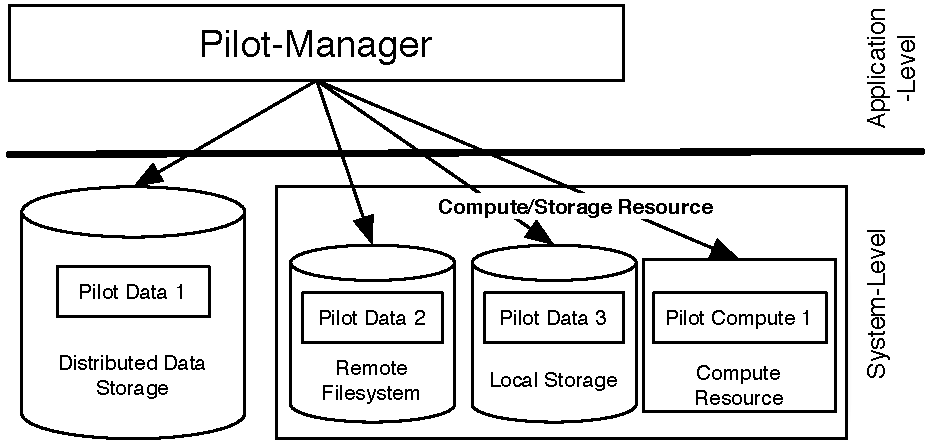
\includegraphics[width=0.7\textwidth]{figures/storage-types.pdf}
	\caption{Pilot-Compute and Pilot-Data on Different Types of Storage Resources}
	\label{fig:figures_storage-types}
\end{figure}

Table~\ref{tab:storage-systems} shows an overview of distributed storage 
systems. The focus of this analysis are file-based storage systems. Structured
storage types (e.g. relational databases) and key-/values stores are not 
considered.

\begin{table}[t]
\centering
\begin{tabular}{|p{2cm}|p{1.2cm}|p{1.2cm}|p{1.2cm}|p{1.2cm}|p{1.2cm}|}
	\hline
	\textbf{Storage Type} &\textbf{Azure} &\textbf{Amazon} &\textbf{Google} &\textbf{XSEDE}  &\textbf{OSG} \\
	\hline
	Local	&yes &yes &yes &yes &yes\\
	\hline
	Network Filesystem &Azure Drive &EBS &GCE Block Storage &Lustre, GPFS 
	&no\\
	\hline
	Distributed Storage &Azure Blob Storage &S3 &Google Storage &GFFS
	 &SRM\\
	\hline	
\end{tabular}
\caption{File-based storage types for different infrastructures (key/value and 
SQL-based storage types omitted) \label{tab:storage-systems}}
\end{table}

\section{Hadoop in the Cloud}

\begin{itemize}
	\item Elastic MapReduce
	\item Hadoop on Azure
\end{itemize}

\section{Pilot Abstractions and Clouds}

% Intro to P* model

\begin{figure}[t]
	\centering
		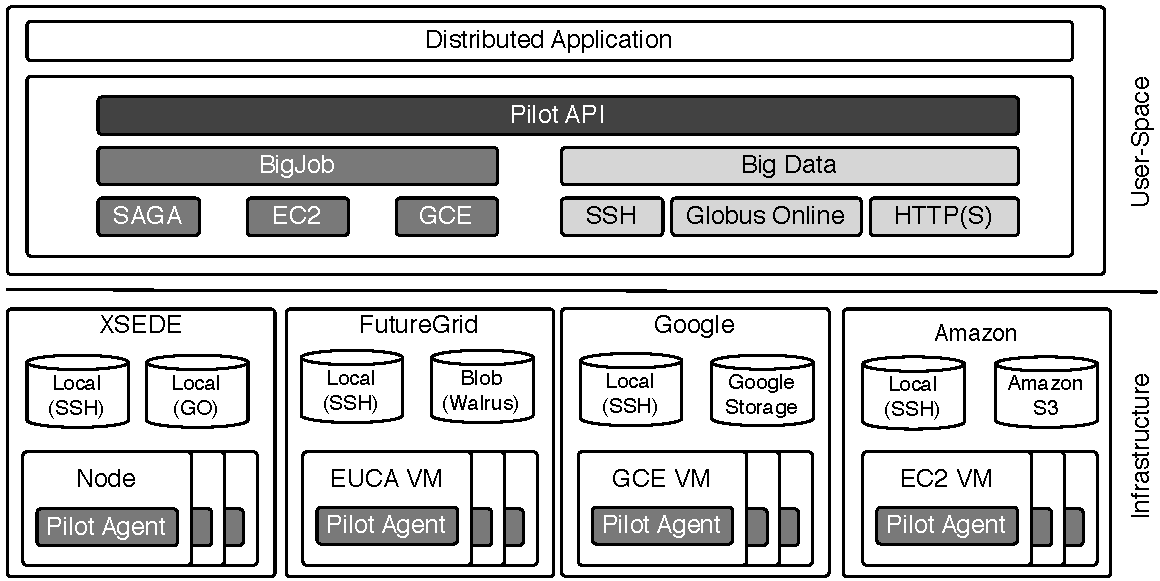
\includegraphics[width=0.7\textwidth]{figures/cloud_pilot_job.pdf}
	\caption{Pilot Abstractions and Clouds}
	\label{fig:figures_cloud_pilot_job}
\end{figure}
Figure~\ref{fig:figures_cloud_pilot_job} shows how the Pilot-API and 
BigJob/BigData can be used to manage a heterogenous set of both cloud and grid 
resources. BigJob supports various resource types via a flexible plugin 
architecture. In addition to SAGA, BJ can natively utilize both the EC2 and 
GCE API to launch BJ agents. Similarly, BigData supports various data access
protocols and storage types -- currently, SSH, Globus Online, Google Storage
and Amazon S3.



Figure~\ref{fig:figures_data-flow} shows the interactions and the data flow 
between Pilot Computes and Data.
\begin{figure}[htbp]
	\centering
		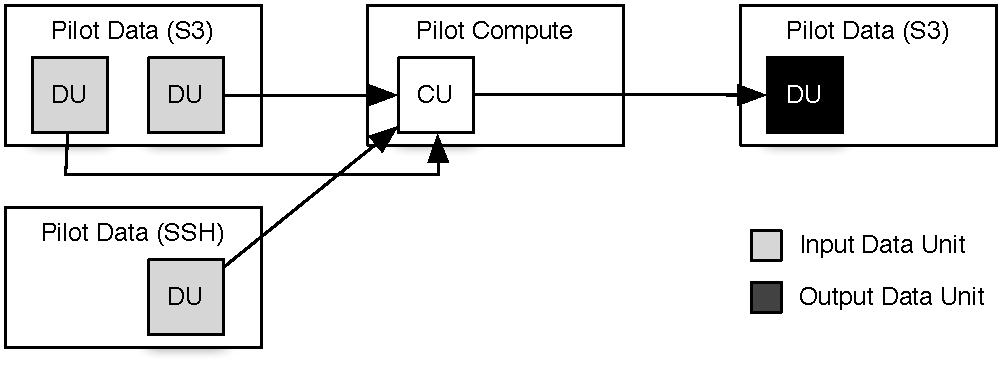
\includegraphics[width=0.7\textwidth]{figures/data-flow.pdf}
	\caption{DU and CU Interactions and Data Flow}
	\label{fig:figures_data-flow}
\end{figure}

\section{Pilot-MapReduce}
Pilot-MapReduce is a pilot-based implementation of the MapReduce
programming model, which decouples the logic/pattern of MapReduce from
the actual management of the compute, data and network resources. By
decoupling job scheduling and monitoring from the resource management,
PMR can efficiently reuse the resource management and late-binding
capabilities of BigJob and BigData.

PMR exposes an easy-to-use interface which provides the complete
functionality needed by any MapReduce-based application, while hiding
the more complex functionality, such as chunking of the input, sorting
the intermediate results, managing and coordinating the map and reduce
tasks, etc., these are generically implemented by the
framework~\cite{pmr2012}.

\section{Experiments}

What Infrastructure?

  - FutureGrid/ XSEDE ( Sierra, Kraken )

  - Eucalyptus Cloud ( Ashley's contributions )
    - Get widely distributed instances. 

  - OpenStack Cloud ( Melissa contributions )
    - Get widely distributed instances. 

Experiments -

  - Scale data 1GB, 10GB, 100GB, 1000 GB
  - Scale Resources 1000 cores, 10000 cores, 50,000 cores

\section{Future Work}

\bibliographystyle{wileyj}
\bibliography{literatur,saga,saga-related,local}

\end{document}
